% Content below is autogenerated 
\subsection{Technical details on low-power jammer 'S1.1'}
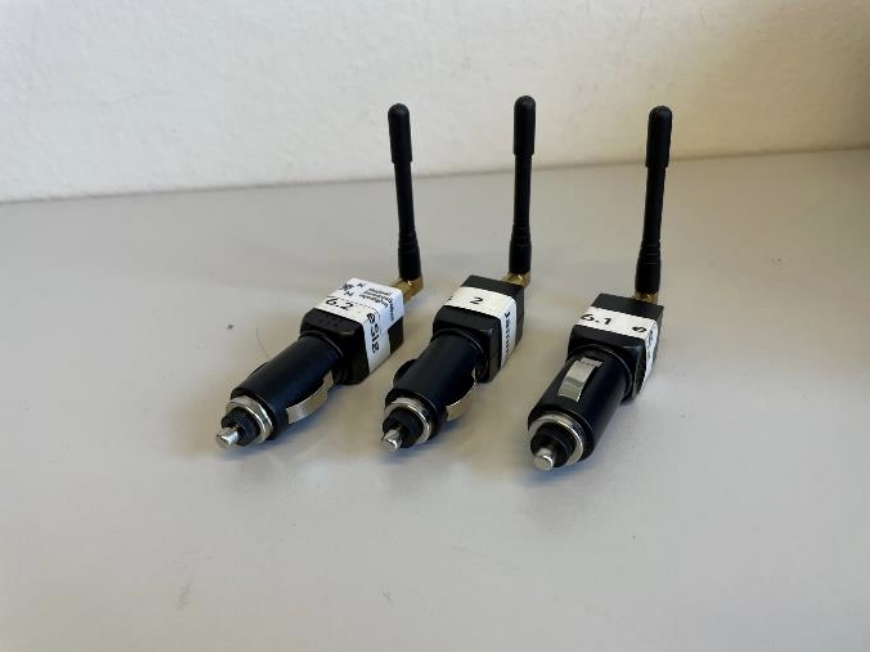
\includegraphics[scale=0.4]{../graphics/appendixG/s1.1-photo.png}\\ \\ 
The jammer S1.1 belongs to the 'Cigarette jammer' category of jammers. Such jammers are often installed in the cigarette lighter outlet in cars. They are intended to cover the car, and a given radius around the car. \\S1.1 is an one-antenna, so-called 'L1-only', jammer, disrupting only the upper L-band.\\
\begin{table}[H]\centering
\begin{tabular}{|c|c|c|c|c|c|c|}\rowcolor[HTML]{C0C0C0} 
\hline
\makecell{Centre frequency\\{[MHz]}} & \makecell{Bandwidth\\{[MHz]}} & \makecell{PSD\\{[dBm/MHz]}} & \makecell{TX total\\{[dBm]}} & \makecell{CF max\\{[dBm]}} & \makecell{Sweep rate\\{[µs]}} & \makecell{Modulation}\\ 
\hline
\makecell{1577.40} & \makecell{29.96} & \makecell{7.58} & \makecell{22.34} & \makecell{7.89} & \makecell{37.1} & \makecell{Sawtooth}\\ 
\hline\end{tabular}\caption{Technical characteristics of S1.1 jammer}\label{table:tech_char_S1.1}\end{table}
\begin{figure}[H]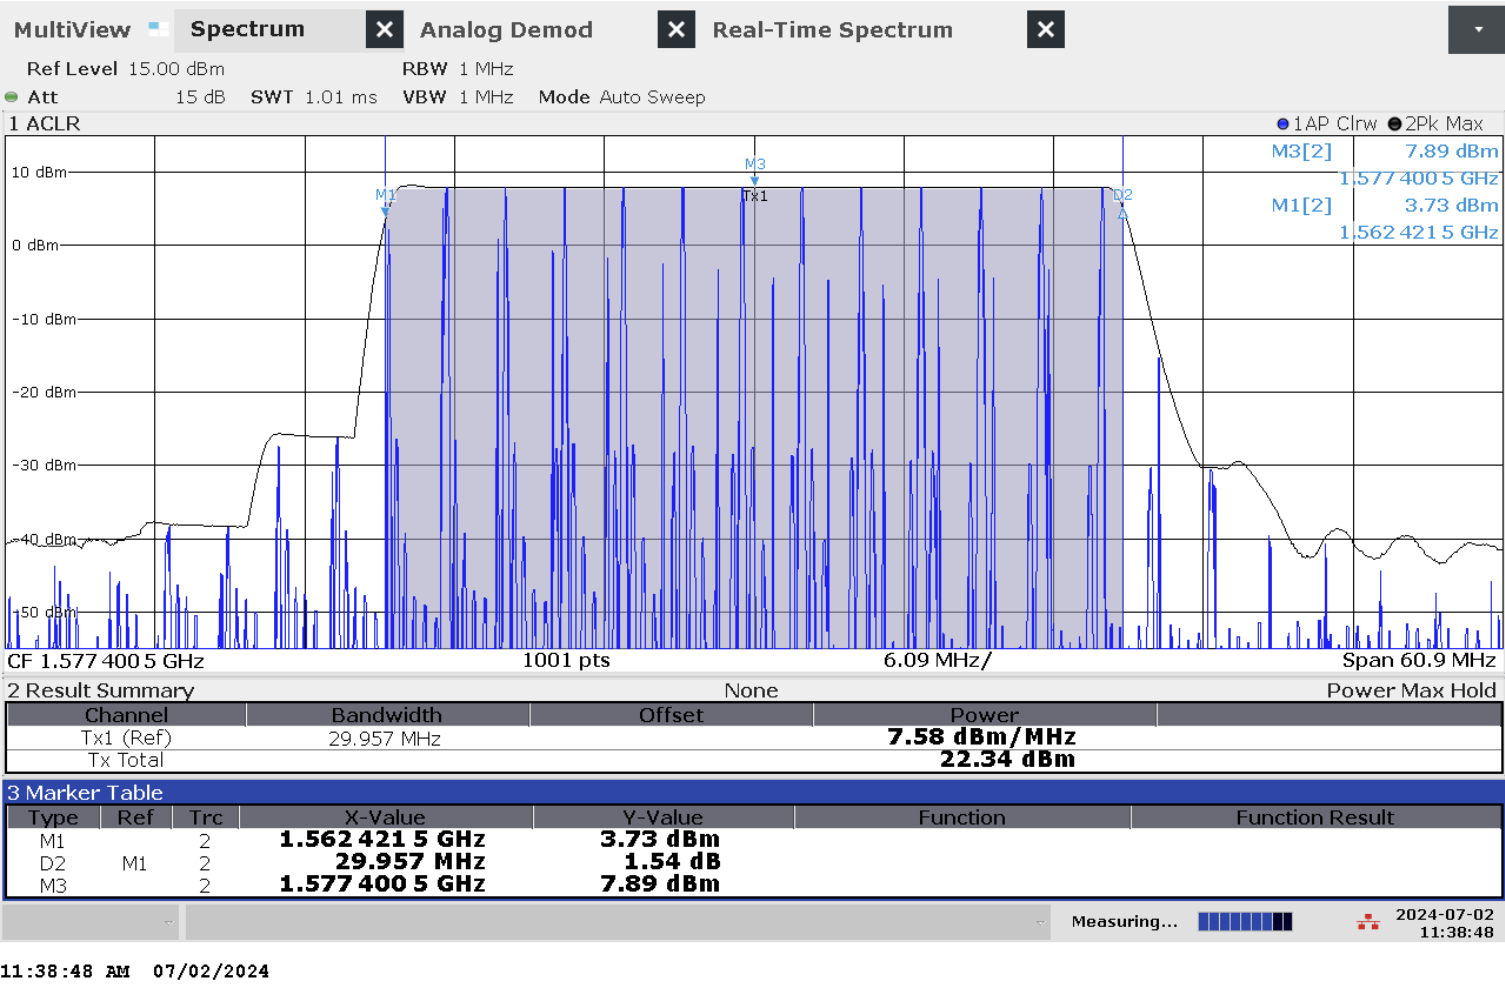
\includegraphics[scale=0.4]{../graphics/appendixG/s1.1-1.png} 
\caption{Frequency and power measurement of jammer S1.1}\end{figure}\begin{figure}[H]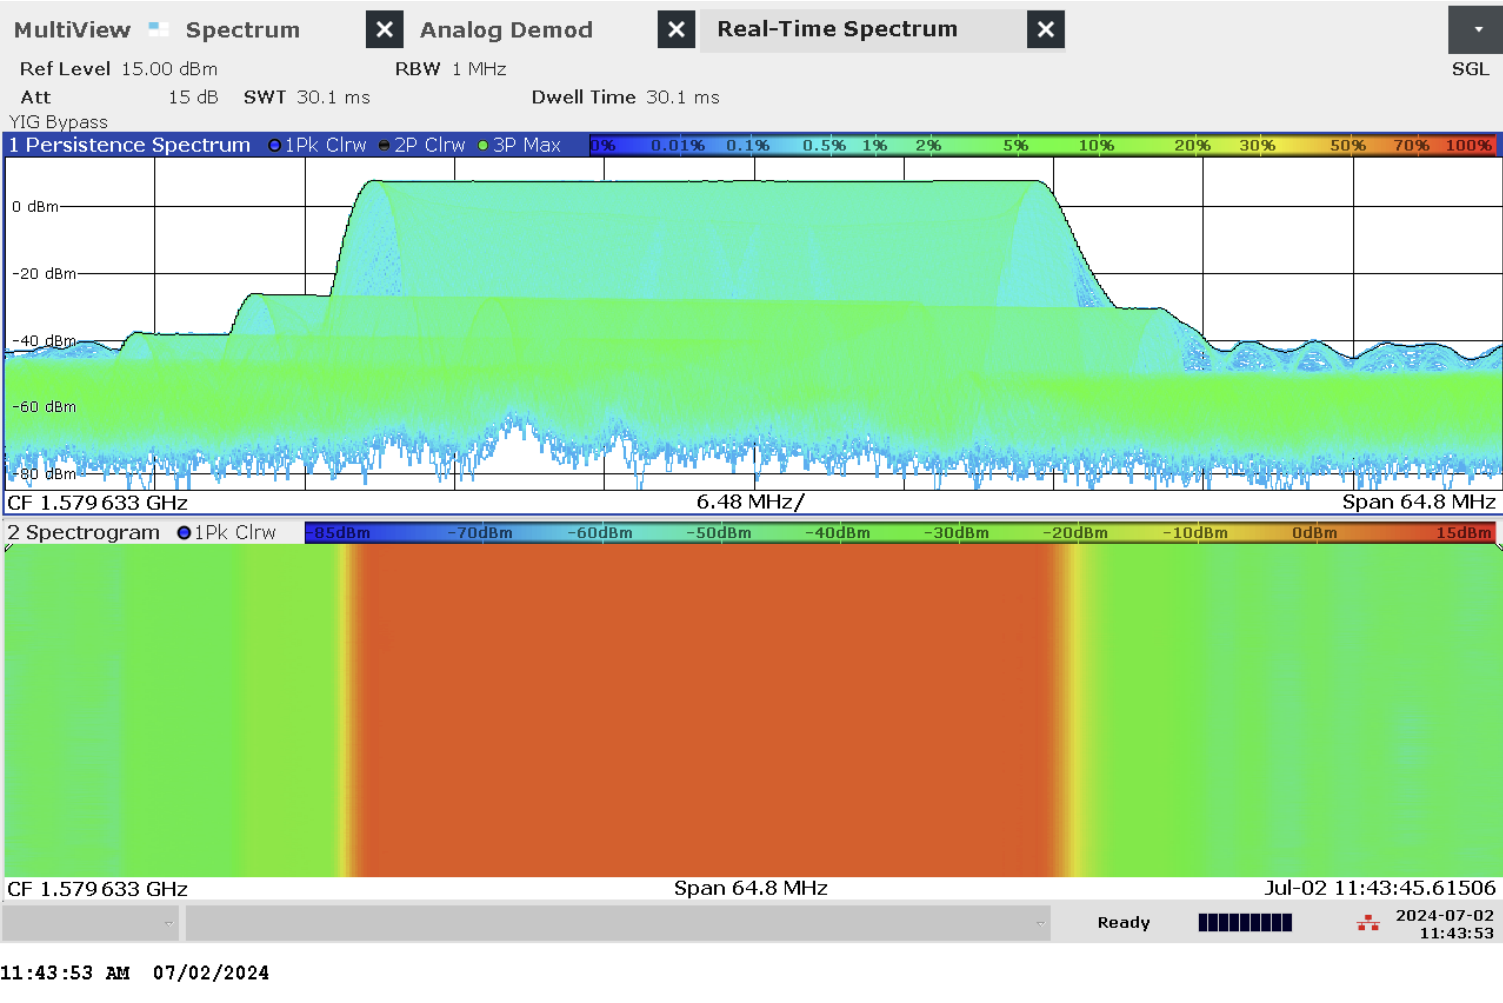
\includegraphics[scale=0.4]{../graphics/appendixG/s1.1-2.png} 
\caption{Real-time persistence and spectrogram measurement of jammer S1.1}\end{figure}\begin{figure}[H]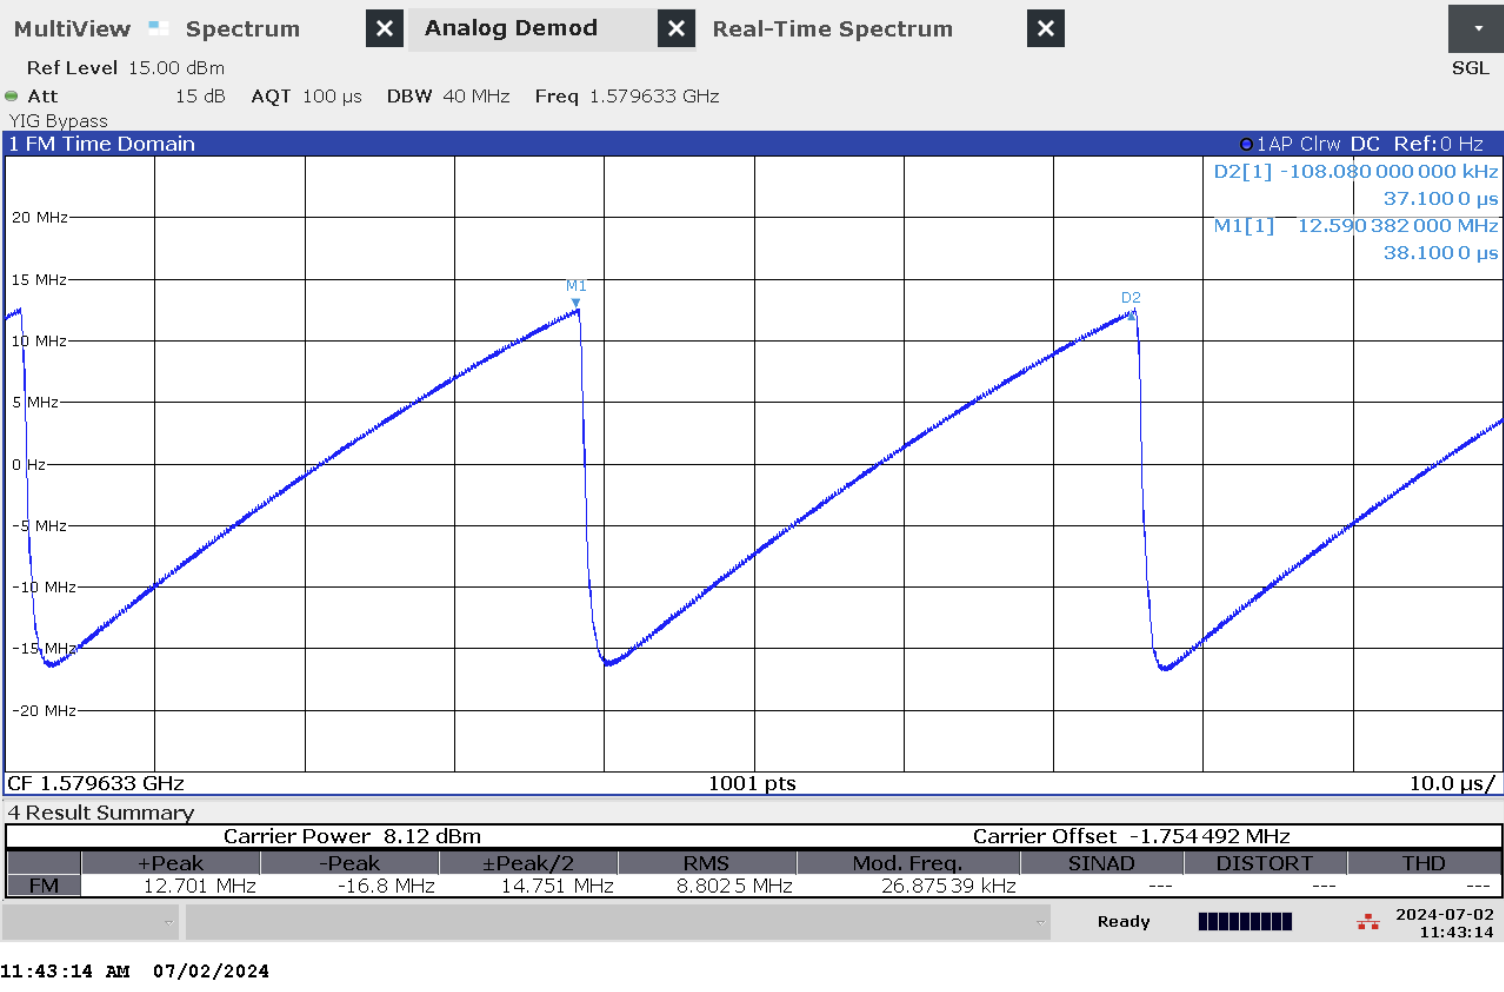
\includegraphics[scale=0.4]{../graphics/appendixG/s1.1-3.png} 
\caption{Time domain (analog demod) measurement of jammer S1.1}\end{figure}\subsection{Technical details on low-power jammer 'S1.2'}
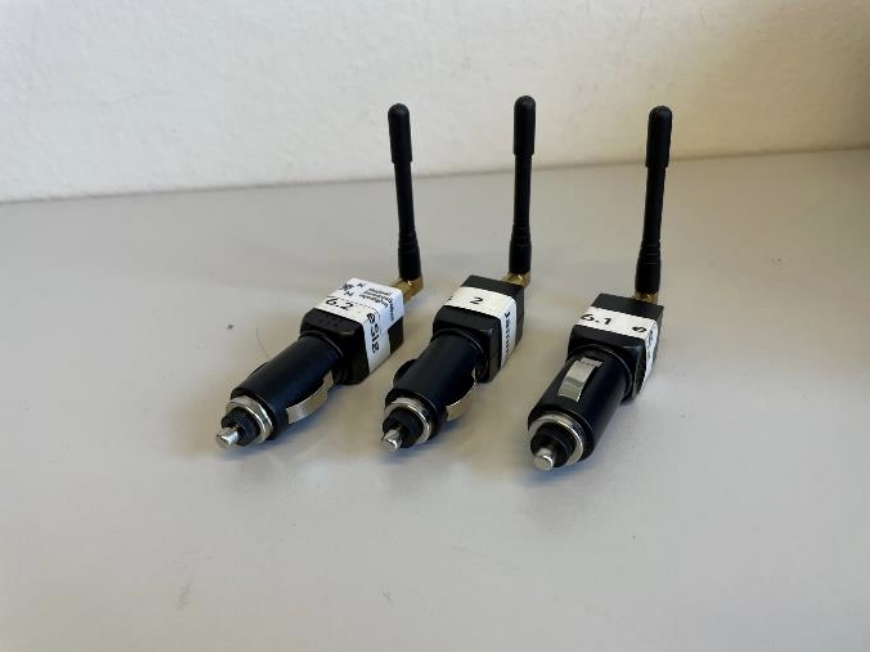
\includegraphics[scale=0.4]{../graphics/appendixG/s1.1-photo.png}\\ \\ 
The jammer S1.2 belongs to the 'Cigarette jammer' category of jammers. Such jammers are often installed in the cigarette lighter outlet in cars. They are intended to cover the car, and a given radius around the car. \\S1.2 is an one-antenna, so-called 'L1-only', jammer, disrupting only the upper L-band.\\
\begin{table}[H]\centering
\begin{tabular}{|c|c|c|c|c|c|c|}\rowcolor[HTML]{C0C0C0} 
\hline
\makecell{Centre frequency\\{[MHz]}} & \makecell{Bandwidth\\{[MHz]}} & \makecell{PSD\\{[dBm/MHz]}} & \makecell{TX total\\{[dBm]}} & \makecell{CF max\\{[dBm]}} & \makecell{Sweep rate\\{[µs]}} & \makecell{Modulation}\\ 
\hline
\makecell{1582.56} & \makecell{40.03} & \makecell{12.38} & \makecell{29.01} & \makecell{12.61} & \makecell{21.56} & \makecell{Sawtooth}\\ 
\hline\end{tabular}\caption{Technical characteristics of S1.2 jammer}\label{table:tech_char_S1.2}\end{table}
\begin{figure}[H]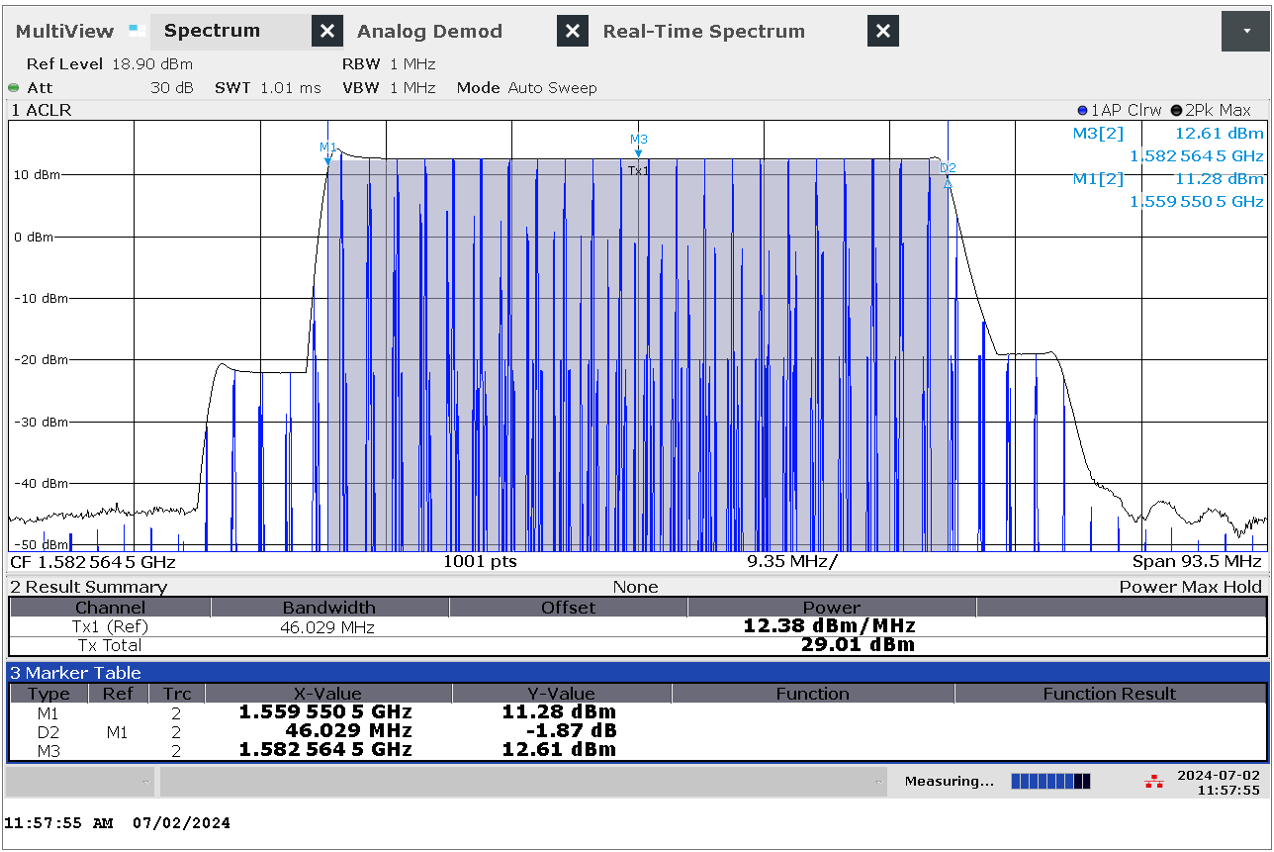
\includegraphics[scale=0.4]{../graphics/appendixG/s1.2-1.png} 
\caption{Frequency and power measurement of jammer S1.2}\end{figure}\begin{figure}[H]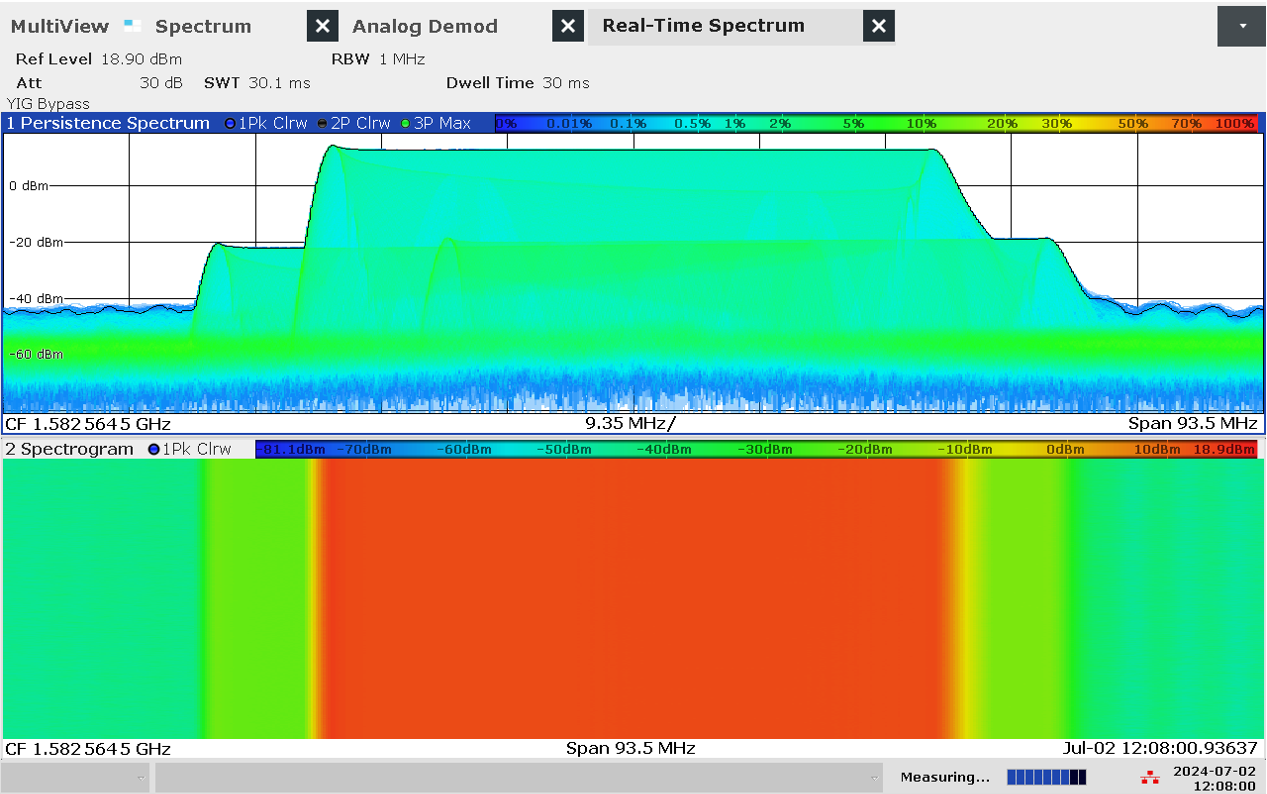
\includegraphics[scale=0.4]{../graphics/appendixG/s1.2-2.png} 
\caption{Real-time persistence and spectrogram measurement of jammer S1.2}\end{figure}\begin{figure}[H]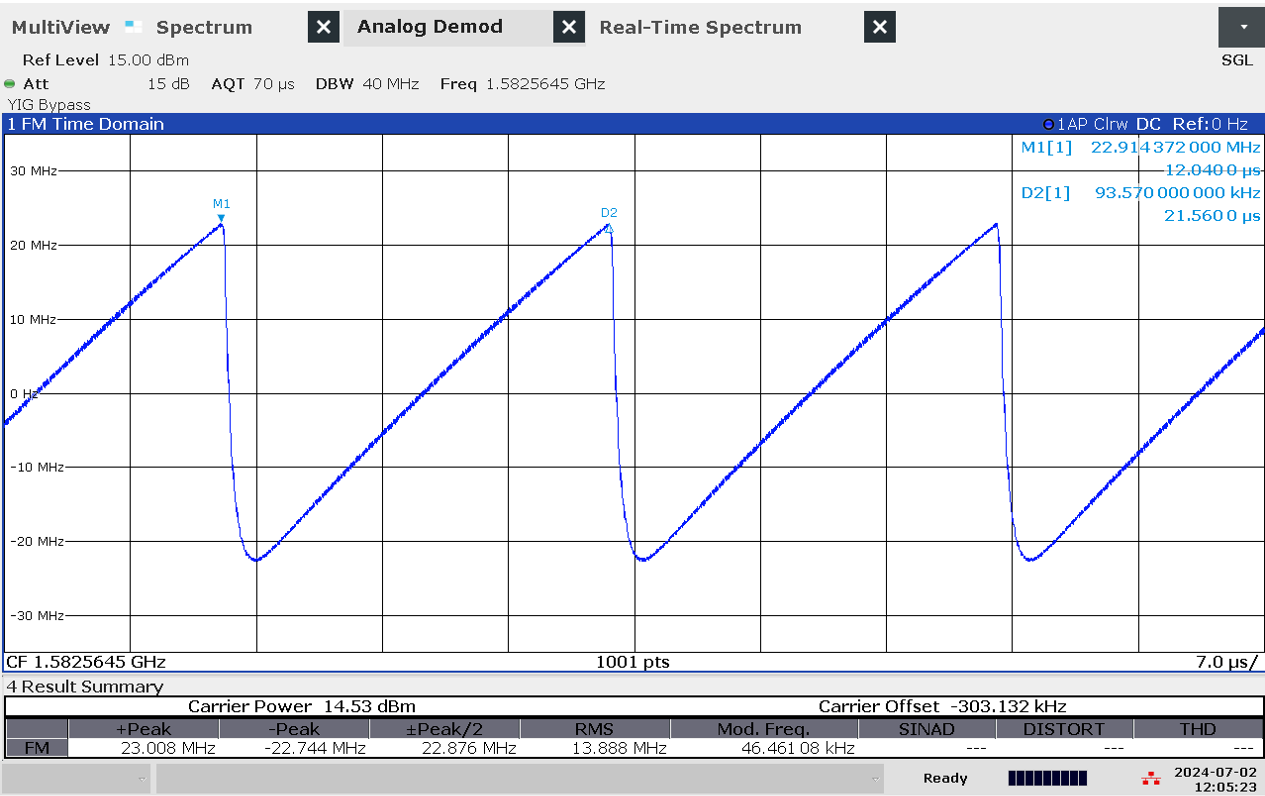
\includegraphics[scale=0.4]{../graphics/appendixG/s1.2-3.png} 
\caption{Time domain (analog demod) measurement of jammer S1.2}\end{figure}\subsection{Technical details on low-power jammer 'S1.3'}
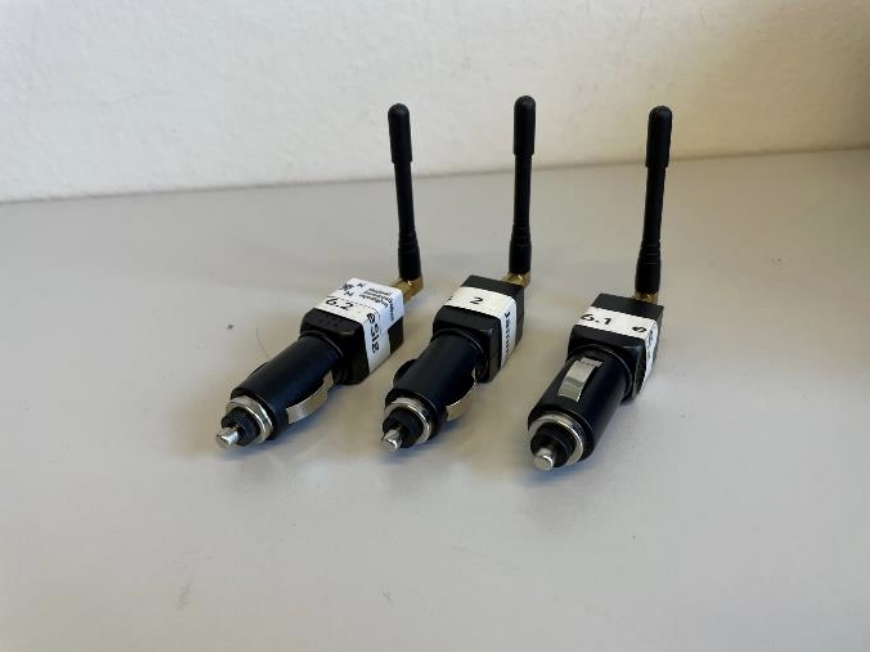
\includegraphics[scale=0.4]{../graphics/appendixG/s1.1-photo.png}\\ \\ 
The jammer S1.3 belongs to the 'Cigarette jammer' category of jammers. Such jammers are often installed in the cigarette lighter outlet in cars. They are intended to cover the car, and a given radius around the car. \\S1.3 is an one-antenna, so-called 'L1-only', jammer, disrupting only the upper L-band.\\
\begin{table}[H]\centering
\begin{tabular}{|c|c|c|c|c|c|c|}\rowcolor[HTML]{C0C0C0} 
\hline
\makecell{Centre frequency\\{[MHz]}} & \makecell{Bandwidth\\{[MHz]}} & \makecell{PSD\\{[dBm/MHz]}} & \makecell{TX total\\{[dBm]}} & \makecell{CF max\\{[dBm]}} & \makecell{Sweep rate\\{[µs]}} & \makecell{Modulation}\\ 
\hline
\makecell{1579.63} & \makecell{31.88} & \makecell{7.56} & \makecell{22.60} & \makecell{7.93} & \makecell{37.5} & \makecell{Sawtooth}\\ 
\hline\end{tabular}\caption{Technical characteristics of S1.3 jammer}\label{table:tech_char_S1.3}\end{table}
\begin{figure}[H]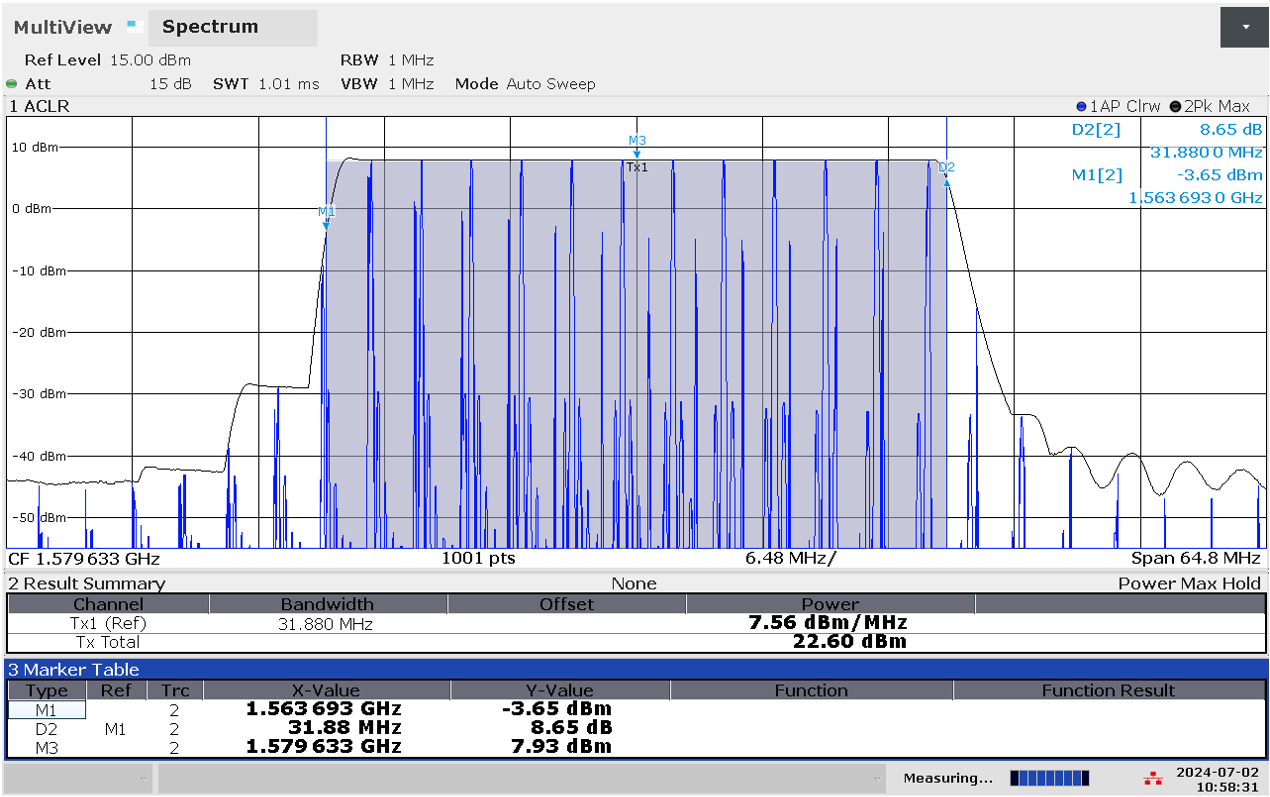
\includegraphics[scale=0.4]{../graphics/appendixG/s1.3-1.png} 
\caption{Frequency and power measurement of jammer S1.3}\end{figure}\begin{figure}[H]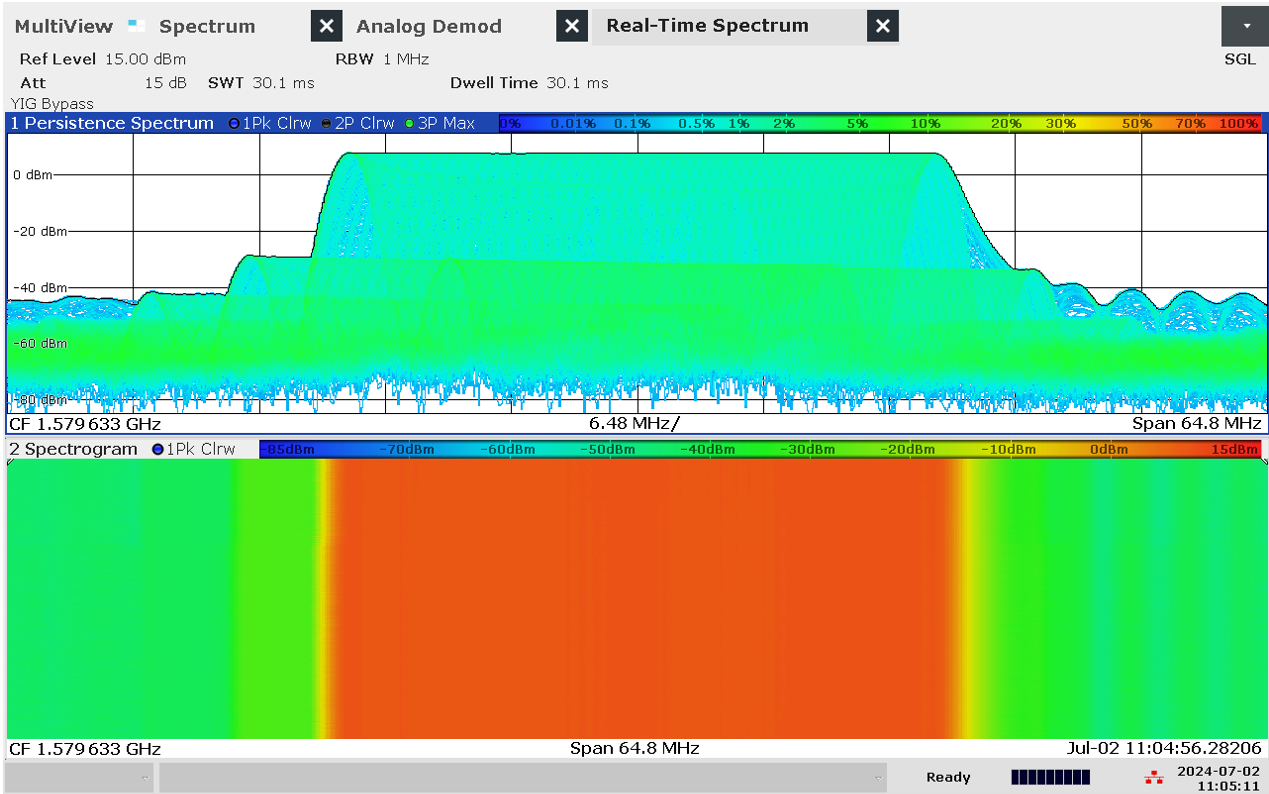
\includegraphics[scale=0.4]{../graphics/appendixG/s1.3-2.png} 
\caption{Real-time persistence and spectrogram measurement of jammer S1.3}\end{figure}\begin{figure}[H]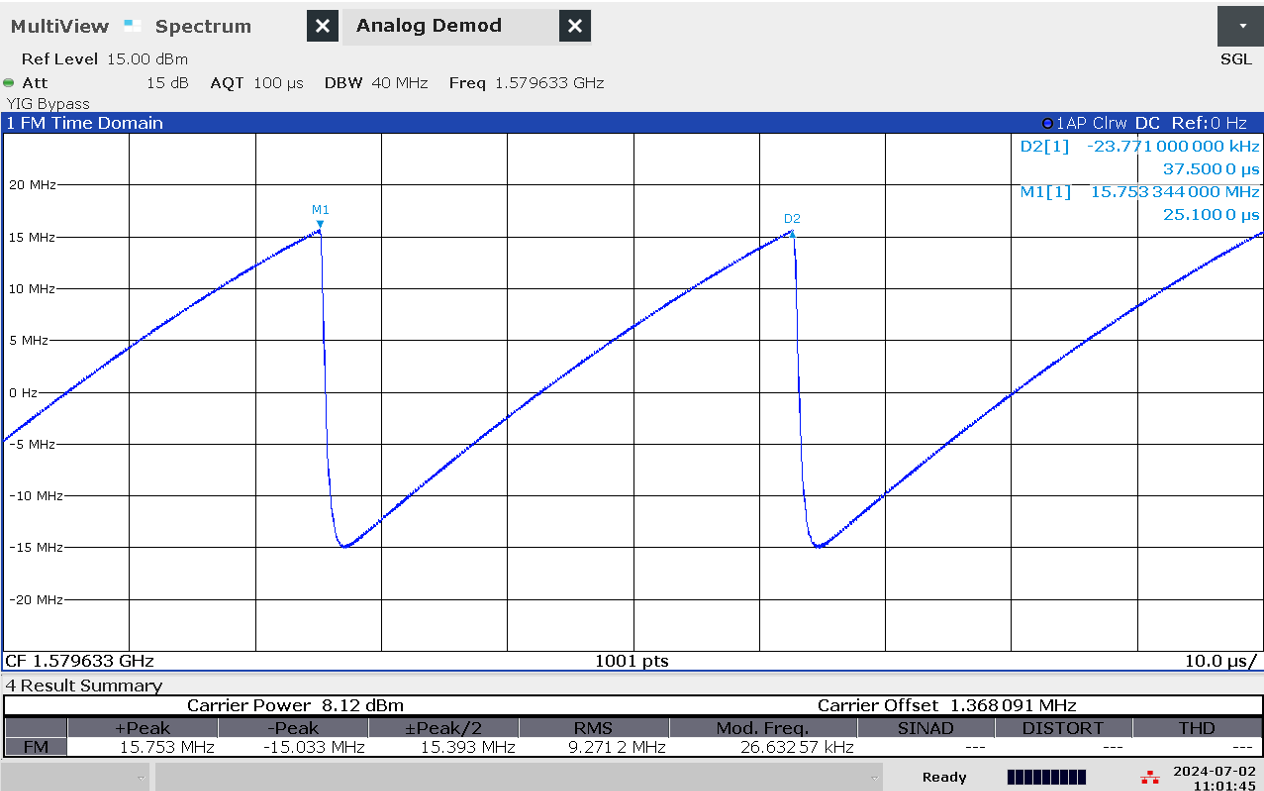
\includegraphics[scale=0.4]{../graphics/appendixG/s1.3-3.png} 
\caption{Time domain (analog demod) measurement of jammer S1.3}\end{figure}\subsection{Technical details on low-power jammer 'S2.1'}
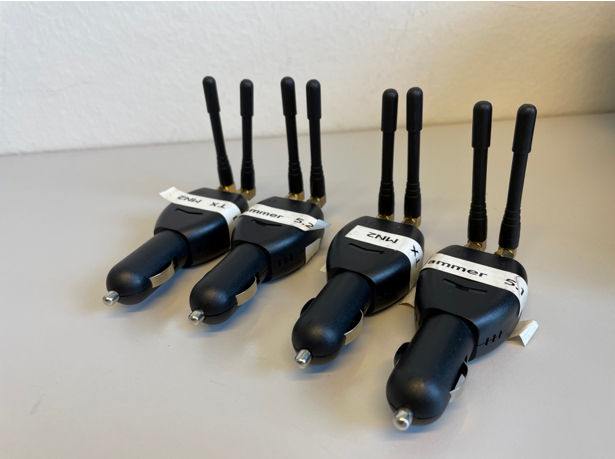
\includegraphics[scale=0.4]{../graphics/appendixG/s2.1-photo.png}\\ \\ 
The jammer S2.1 belongs to the 'Cigarette jammer' category of jammers. Such jammers are often installed in the cigarette lighter outlet in cars. They are intended to cover the car, and a given radius around the car. \\S2.1 is a two-antenna, so-called 'L1+L2', jammer, disrupting both the upper and lower L-band.\\
\begin{table}[H]\centering
\begin{tabular}{|c|c|c|c|c|c|c|c|}\rowcolor[HTML]{C0C0C0} 
\hline
\makecell{Antenna} & \makecell{Centre frequency\\{[MHz]}} & \makecell{Bandwidth\\{[MHz]}} & \makecell{PSD\\{[dBm/MHz]}} & \makecell{TX total\\{[dBm]}} & \makecell{CF max\\{[dBm]}} & \makecell{Sweep rate\\{[µs]}} & \makecell{Modulation}\\ 
\hline
\makecell{L1} & \makecell{1581.59} & \makecell{85.41} & \makecell{13.36} & \makecell{32.68} & \makecell{16.64} & \makecell{40.63} & \makecell{Sawtooth+burst}\\ 
\hline
\makecell{L2} & \makecell{1198.05} & \makecell{96.58} & \makecell{13.92} & \makecell{33.75} & \makecell{17.30} & \makecell{42.1} & \makecell{Sawtooth+burst}\\ 
\hline\end{tabular}\caption{Technical characteristics of S2.1 jammer}\label{table:tech_char_S2.1}\end{table}
\begin{figure}[H]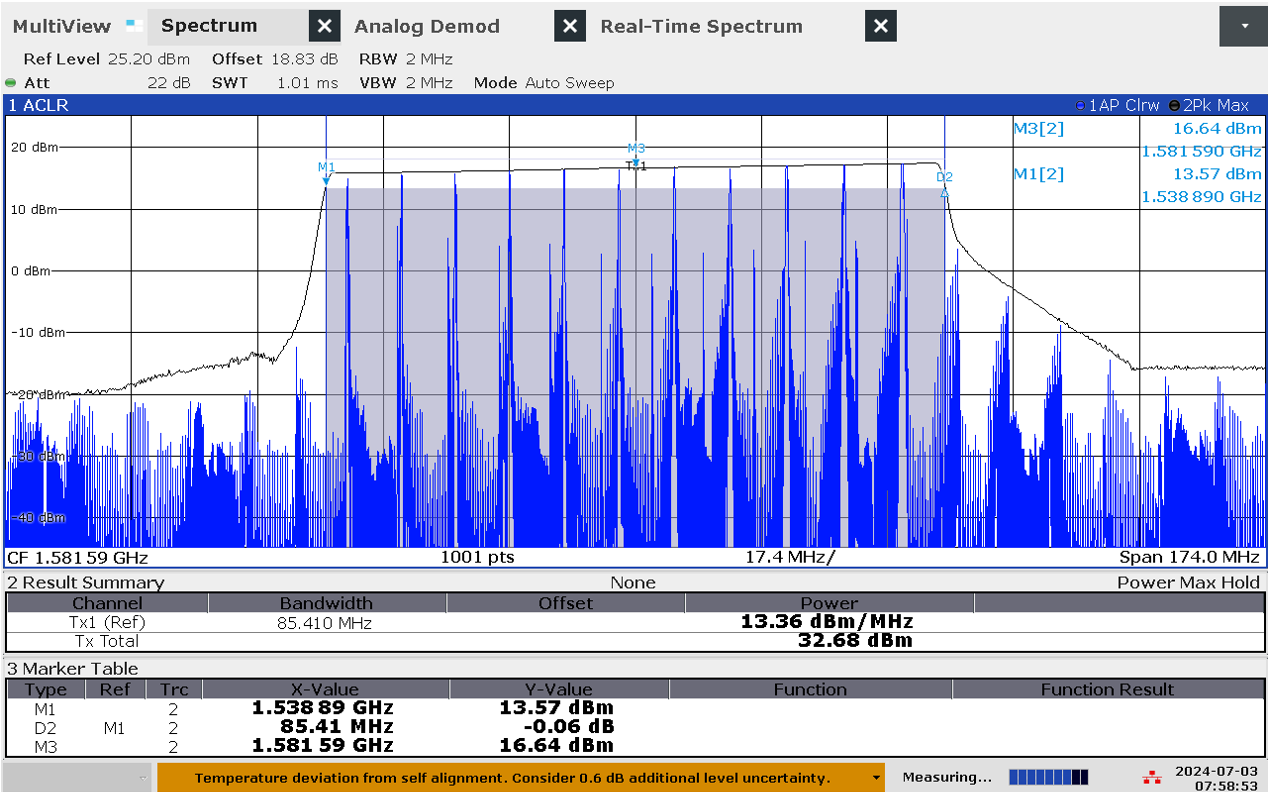
\includegraphics[scale=0.4]{../graphics/appendixG/s2.1-1.png} 
\caption{Frequency and power measurement of jammer S2.1 on antenna 'L1'}\end{figure}\begin{figure}[H]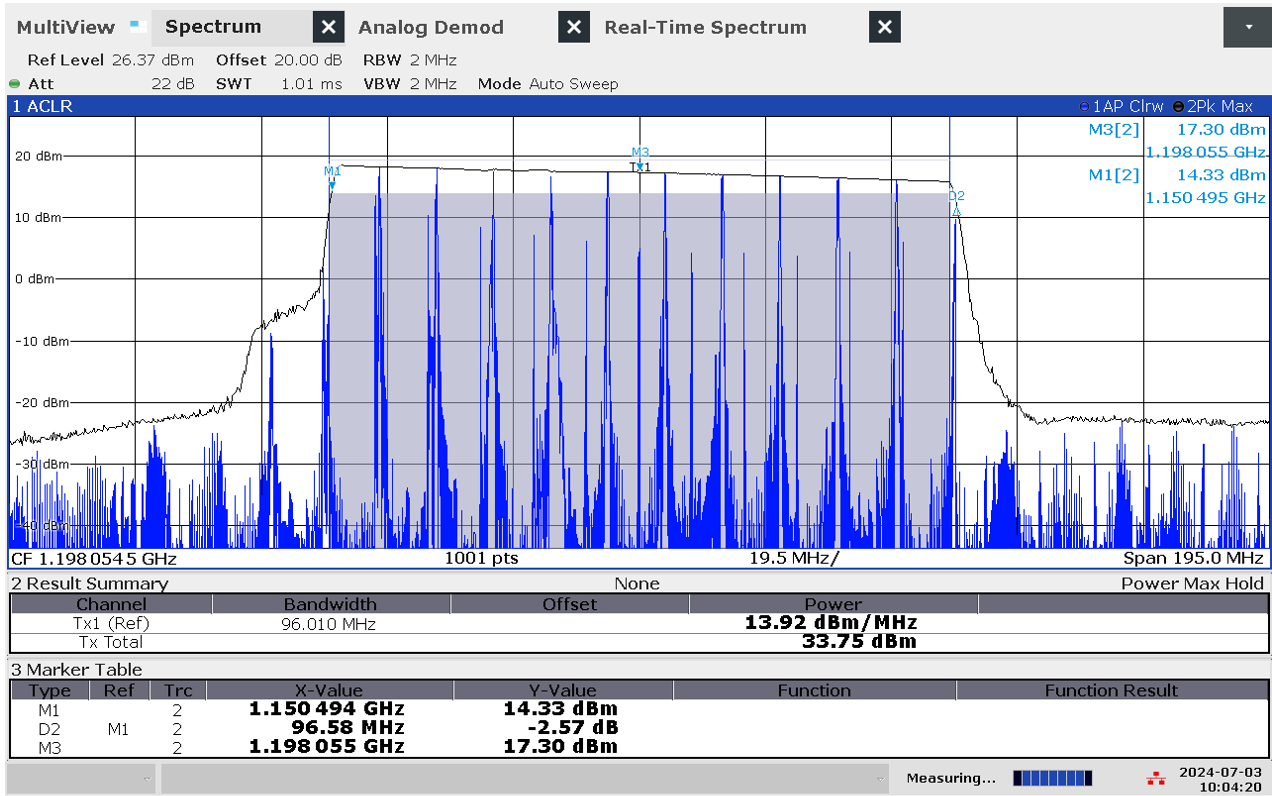
\includegraphics[scale=0.4]{../graphics/appendixG/s2.1-2.png} 
\caption{Frequency and power measurement of jammer S2.1 on antenna 'L2'}\end{figure}\begin{figure}[H]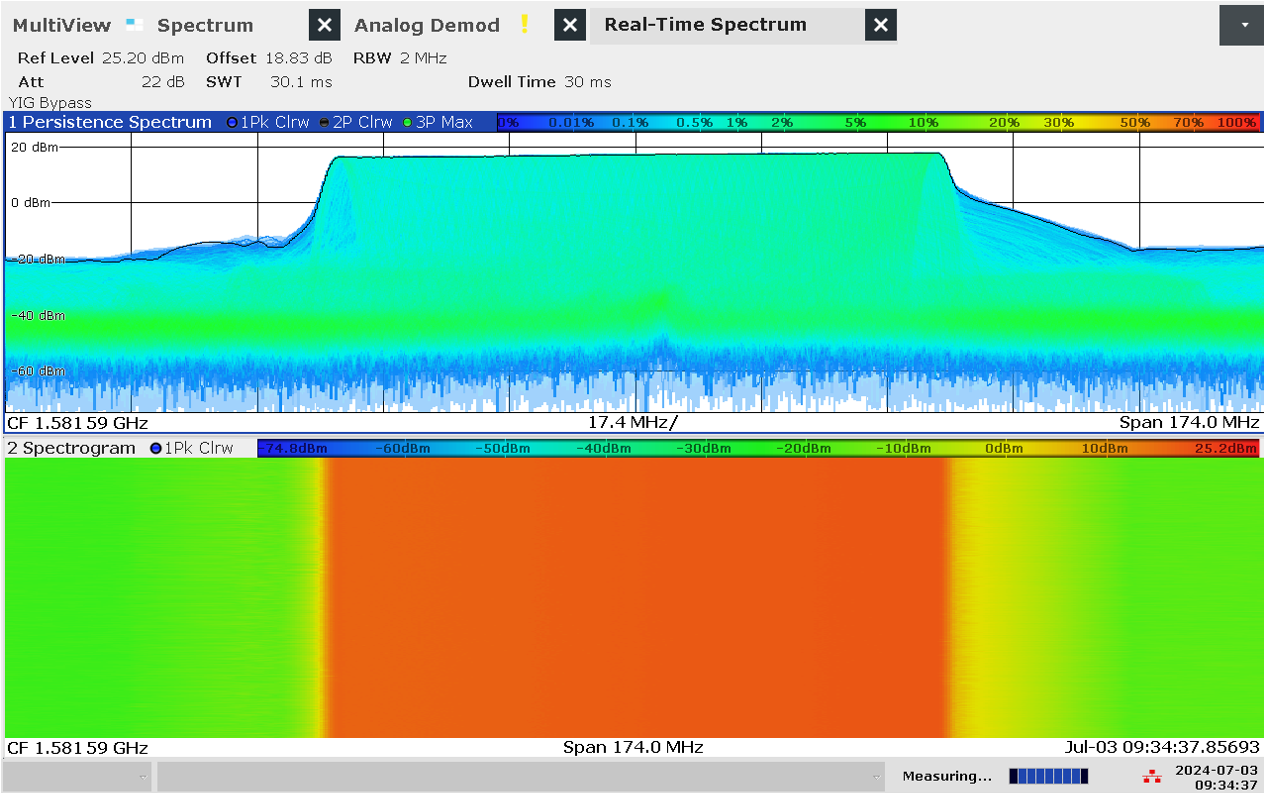
\includegraphics[scale=0.4]{../graphics/appendixG/s2.1-3.png} 
\caption{Real-time persistence and spectrogram measurement of jammer S2.1 on antenna 'L1'}\end{figure}\begin{figure}[H]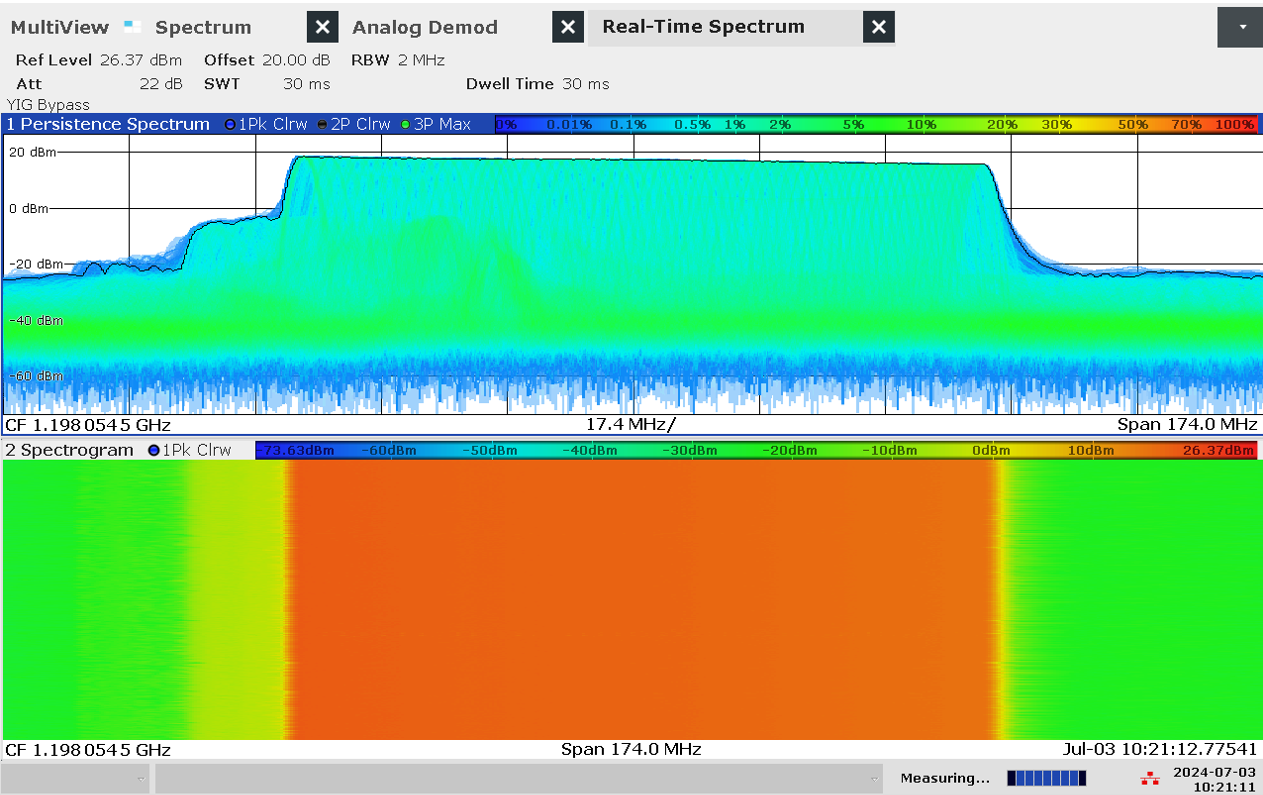
\includegraphics[scale=0.4]{../graphics/appendixG/s2.1-4.png} 
\caption{Real-time persistence and spectrogram measurement of jammer S2.1 on antenna 'L2'}\end{figure}\begin{figure}[H]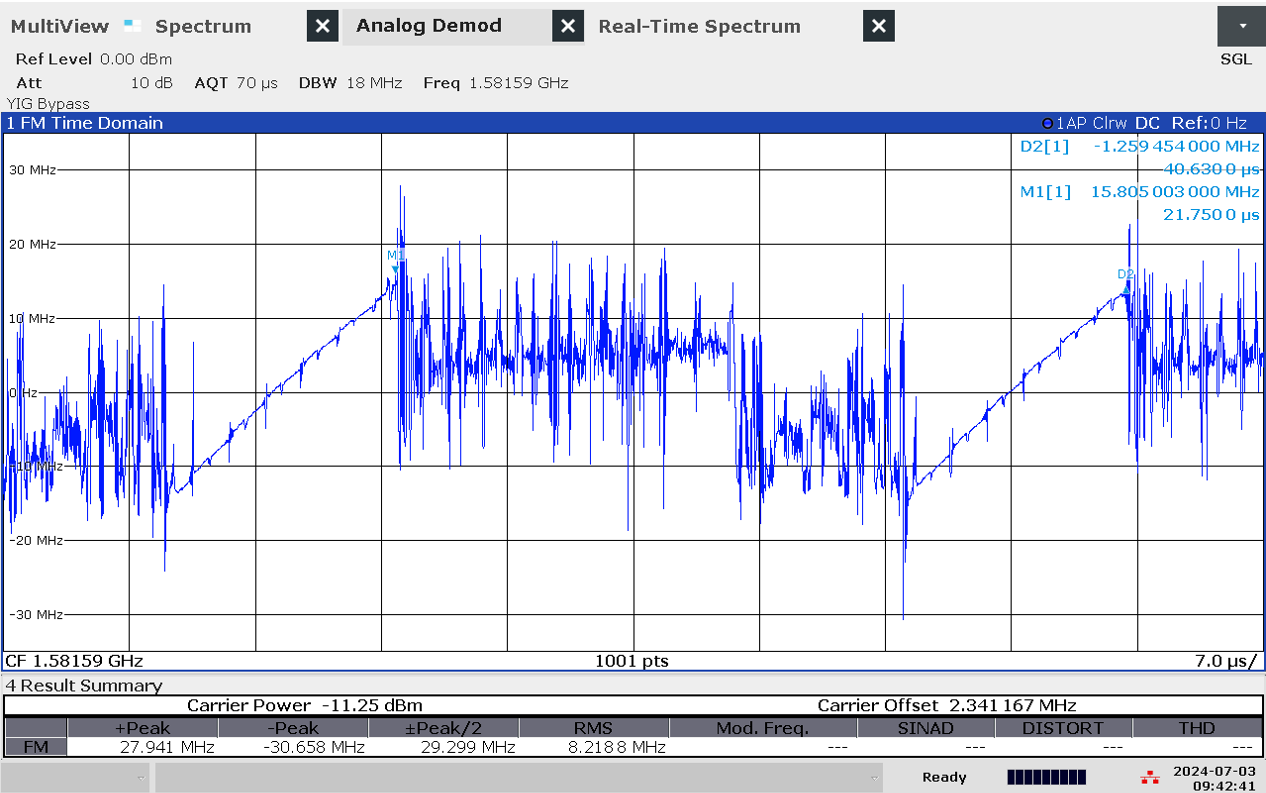
\includegraphics[scale=0.4]{../graphics/appendixG/s2.1-5.png} 
\caption{Time domain (analog demod) measurement of jammer S2.1 on antenna 'L1'}\end{figure}\begin{figure}[H]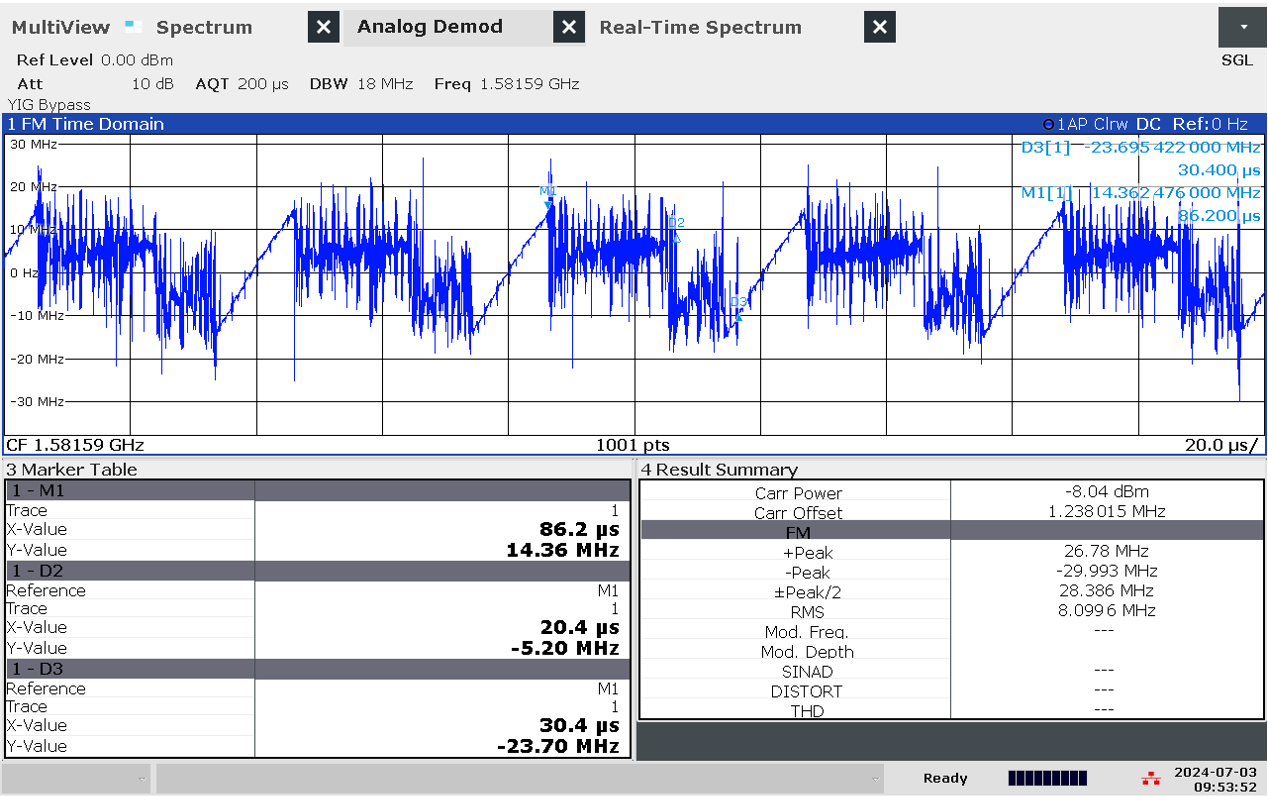
\includegraphics[scale=0.4]{../graphics/appendixG/s2.1-6.png} 
\caption{Time domain (analog demod) measurement with wider span of jammer S2.1 on antenna 'L1'}\end{figure}\begin{figure}[H]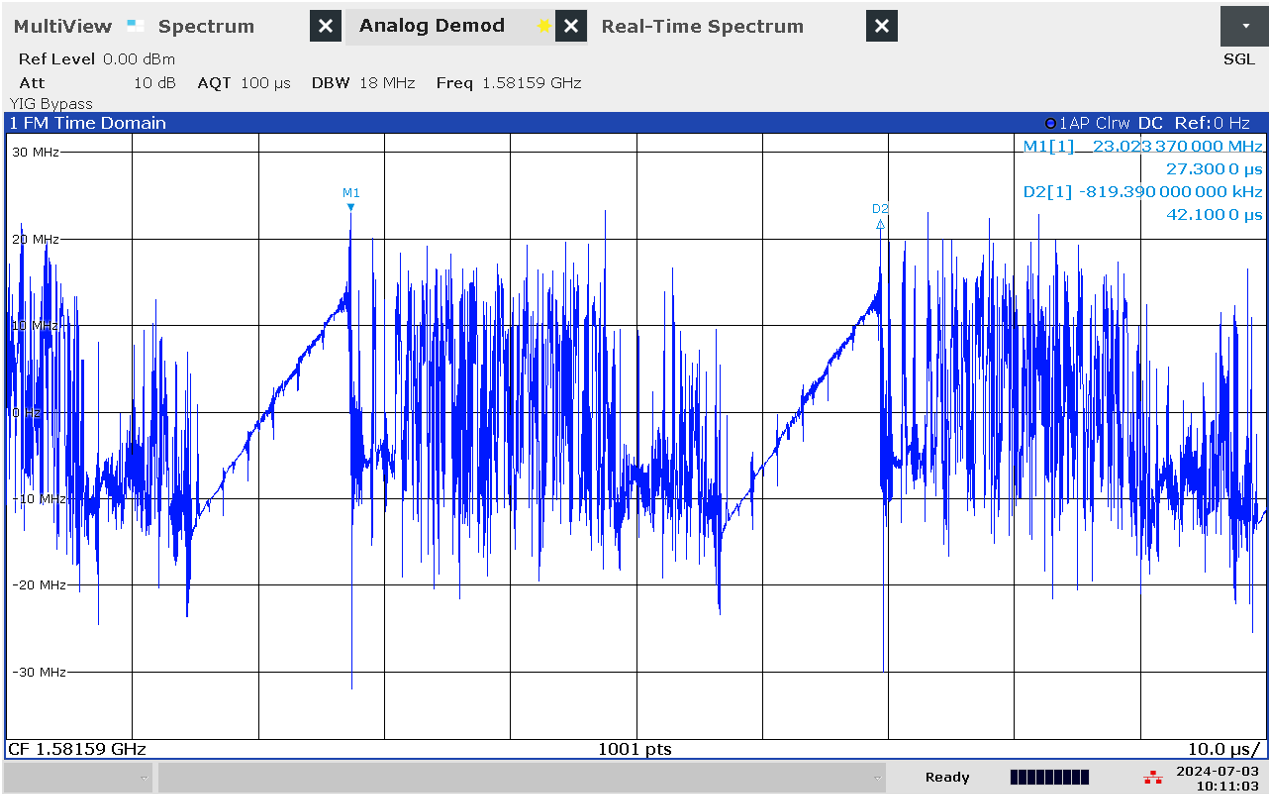
\includegraphics[scale=0.4]{../graphics/appendixG/s2.1-7.png} 
\caption{Time domain (analog demod) measurement of jammer S2.1 on antenna 'L2'}\end{figure}\subsection{Technical details on low-power jammer 'S2.2'}
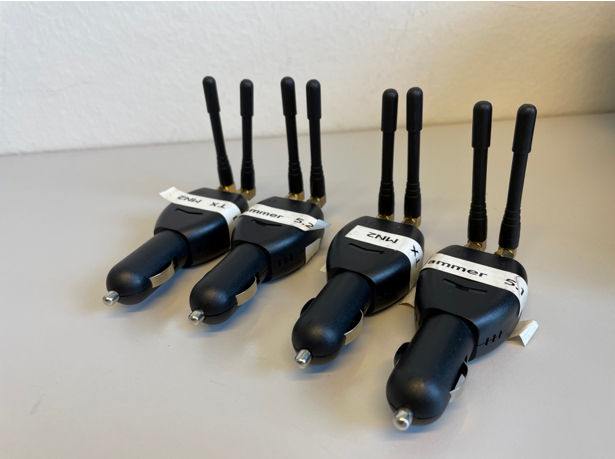
\includegraphics[scale=0.4]{../graphics/appendixG/s2.1-photo.png}\\ \\ 
The jammer S2.2 belongs to the 'Cigarette jammer' category of jammers. Such jammers are often installed in the cigarette lighter outlet in cars. They are intended to cover the car, and a given radius around the car. \\S2.2 is a two-antenna, so-called 'L1+L2', jammer, disrupting both the upper and lower L-band.\\
\begin{table}[H]\centering
\begin{tabular}{|c|c|c|c|c|c|c|c|}\rowcolor[HTML]{C0C0C0} 
\hline
\makecell{Antenna} & \makecell{Centre frequency\\{[MHz]}} & \makecell{Bandwidth\\{[MHz]}} & \makecell{PSD\\{[dBm/MHz]}} & \makecell{TX total\\{[dBm]}} & \makecell{CF max\\{[dBm]}} & \makecell{Sweep rate\\{[µs]}} & \makecell{Modulation}\\ 
\hline
\makecell{L1} & \makecell{1580.86} & \makecell{87.69} & \makecell{12.82} & \makecell{32.25} & \makecell{16.17} & \makecell{40.7} & \makecell{Sawtooth+burst}\\ 
\hline
\makecell{L2} & \makecell{1207.55} & \makecell{102.04} & \makecell{11.95} & \makecell{32.04} & \makecell{17.02} & \makecell{41.0} & \makecell{Sawtooth+burst}\\ 
\hline\end{tabular}\caption{Technical characteristics of S2.2 jammer}\label{table:tech_char_S2.2}\end{table}
\begin{figure}[H]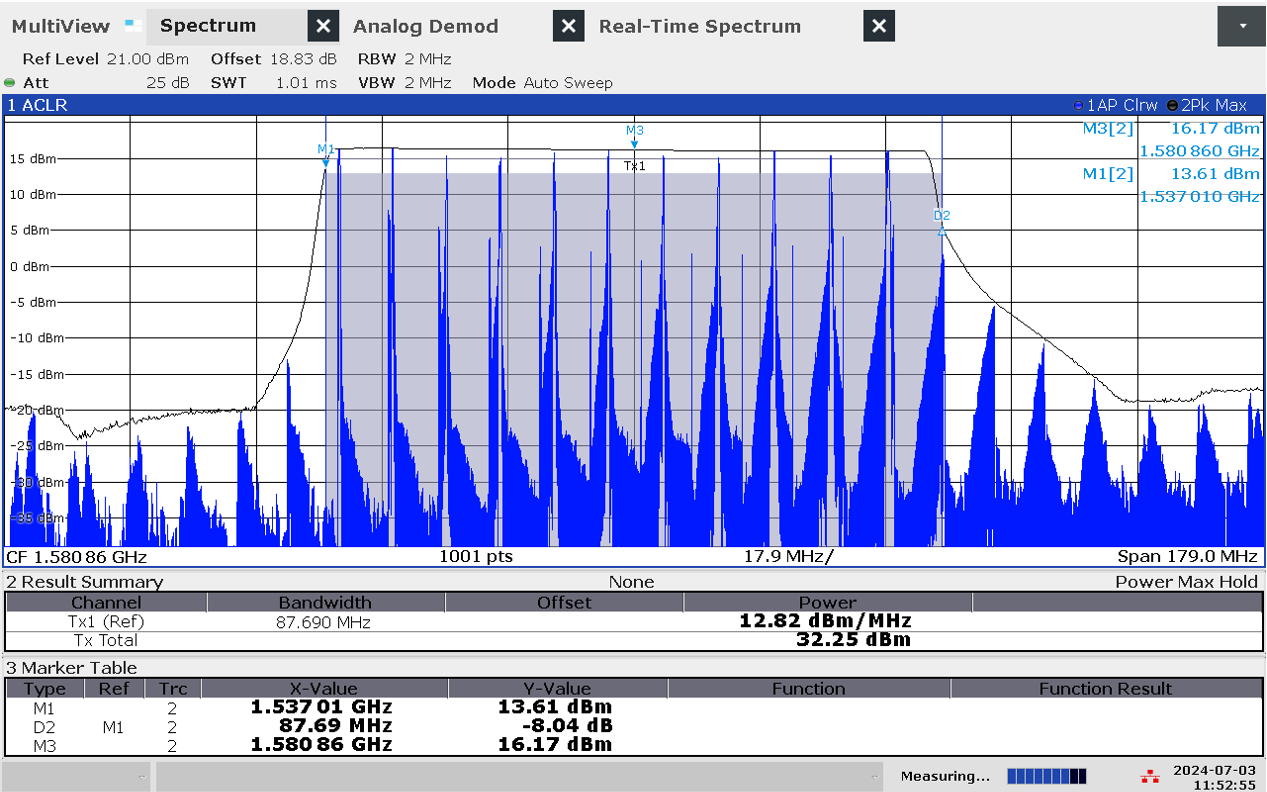
\includegraphics[scale=0.4]{../graphics/appendixG/s2.2-1.png} 
\caption{Frequency and power measurement of jammer S2.2 on antenna 'L1'}\end{figure}\begin{figure}[H]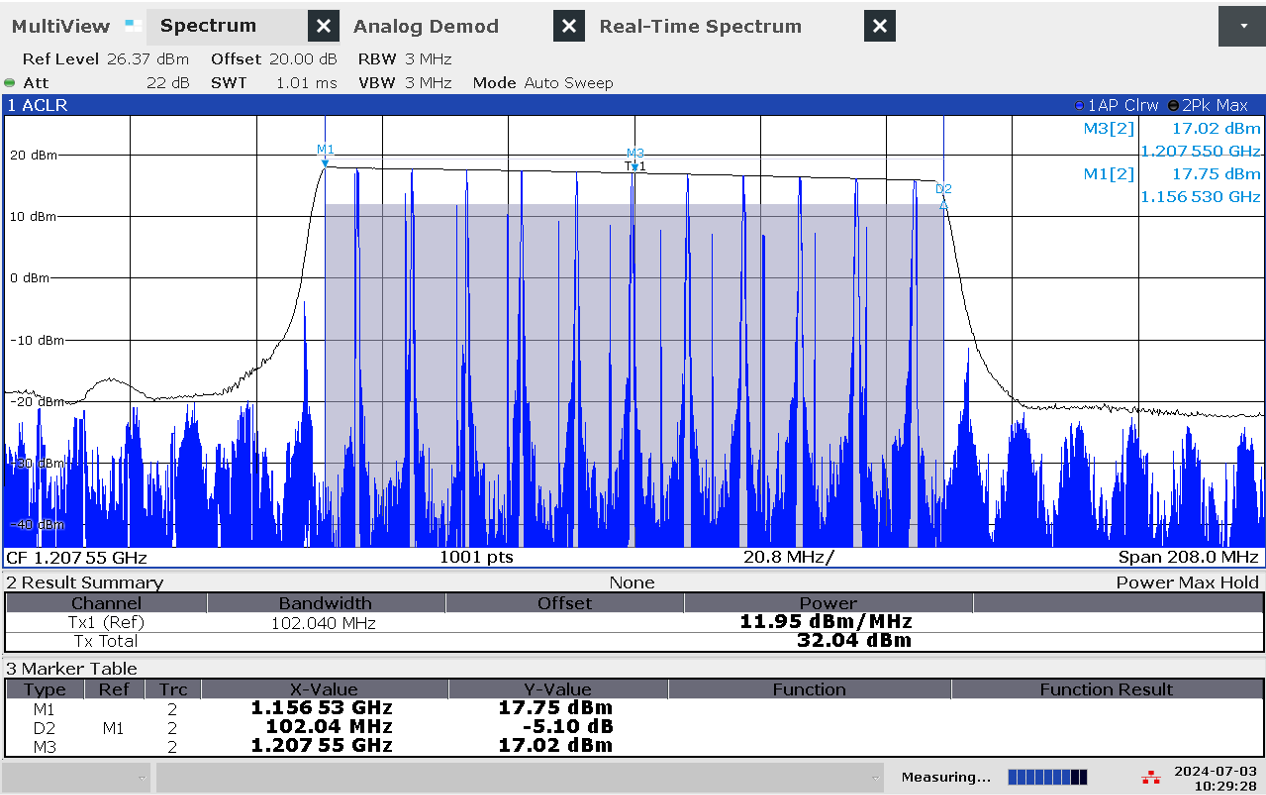
\includegraphics[scale=0.4]{../graphics/appendixG/s2.2-2.png} 
\caption{Frequency and power measurement of jammer S2.2 on antenna 'L2'}\end{figure}\begin{figure}[H]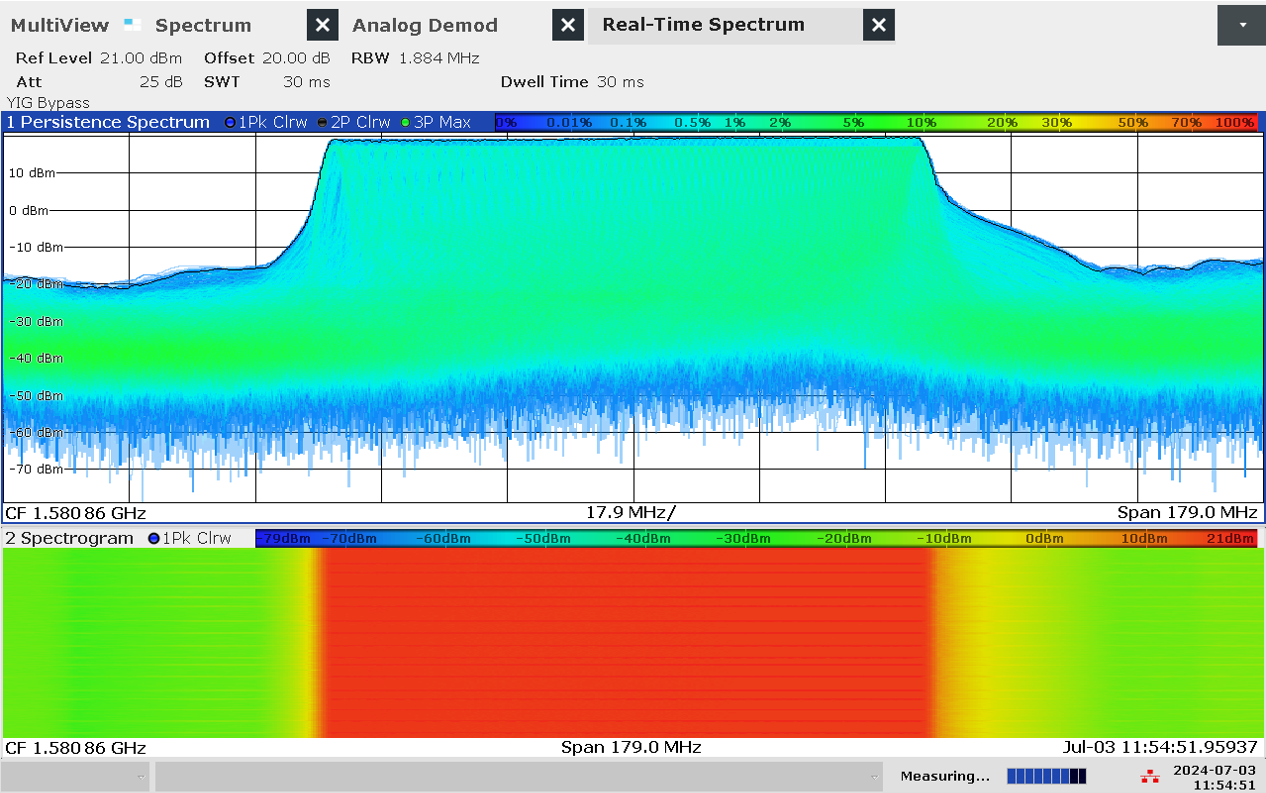
\includegraphics[scale=0.4]{../graphics/appendixG/s2.2-3.png} 
\caption{Real-time persistence and spectrogram measurement of jammer S2.2 on antenna 'L1'}\end{figure}\begin{figure}[H]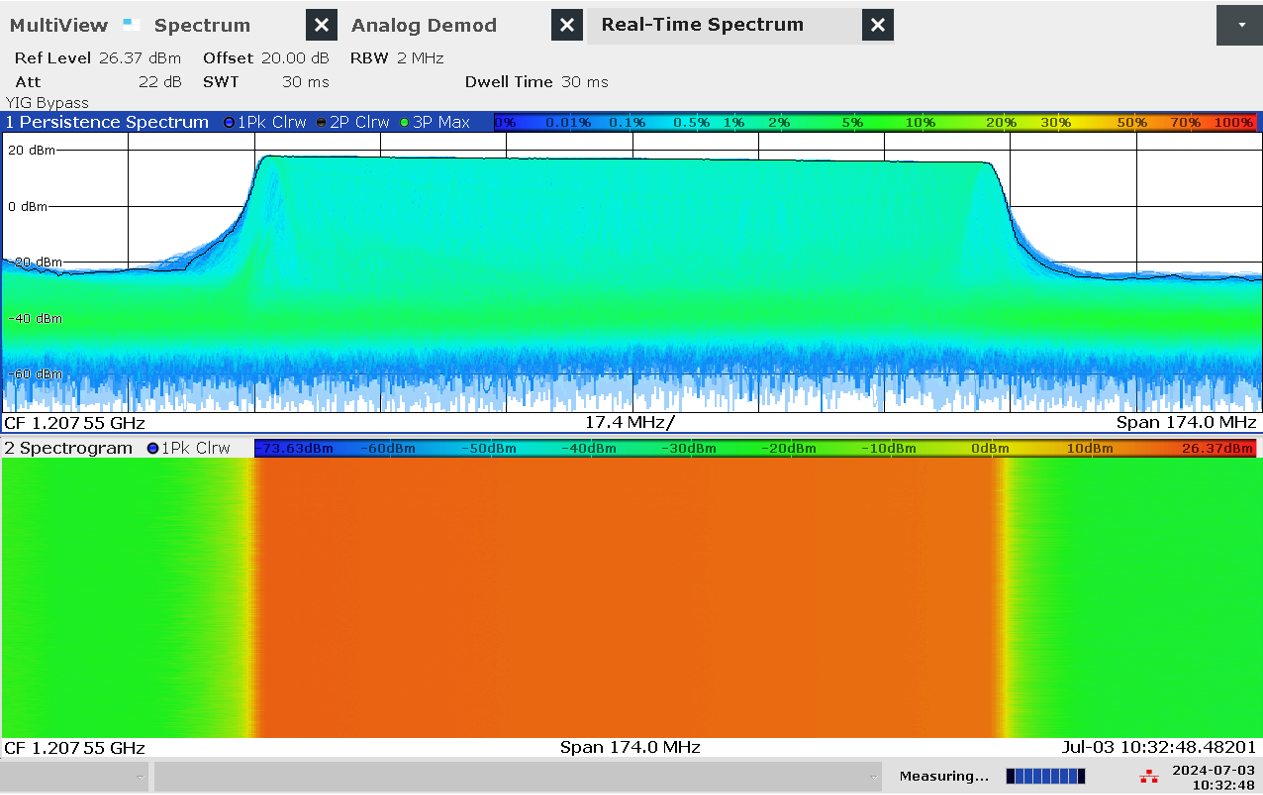
\includegraphics[scale=0.4]{../graphics/appendixG/s2.2-4.png} 
\caption{Real-time persistence and spectrogram measurement of jammer S2.2 on antenna 'L2'}\end{figure}\begin{figure}[H]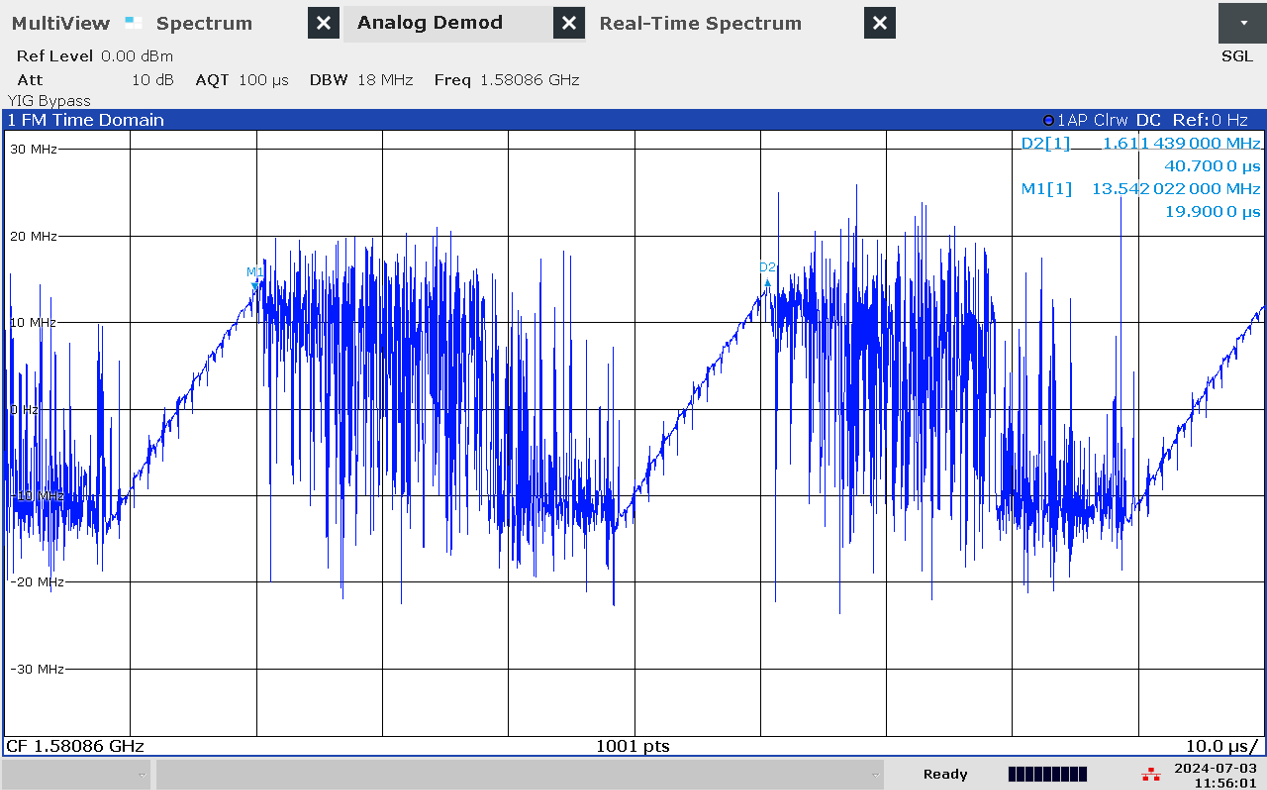
\includegraphics[scale=0.4]{../graphics/appendixG/s2.2-5.png} 
\caption{Time domain (analog demod) measurement of jammer S2.2 on antenna 'L1'}\end{figure}\begin{figure}[H]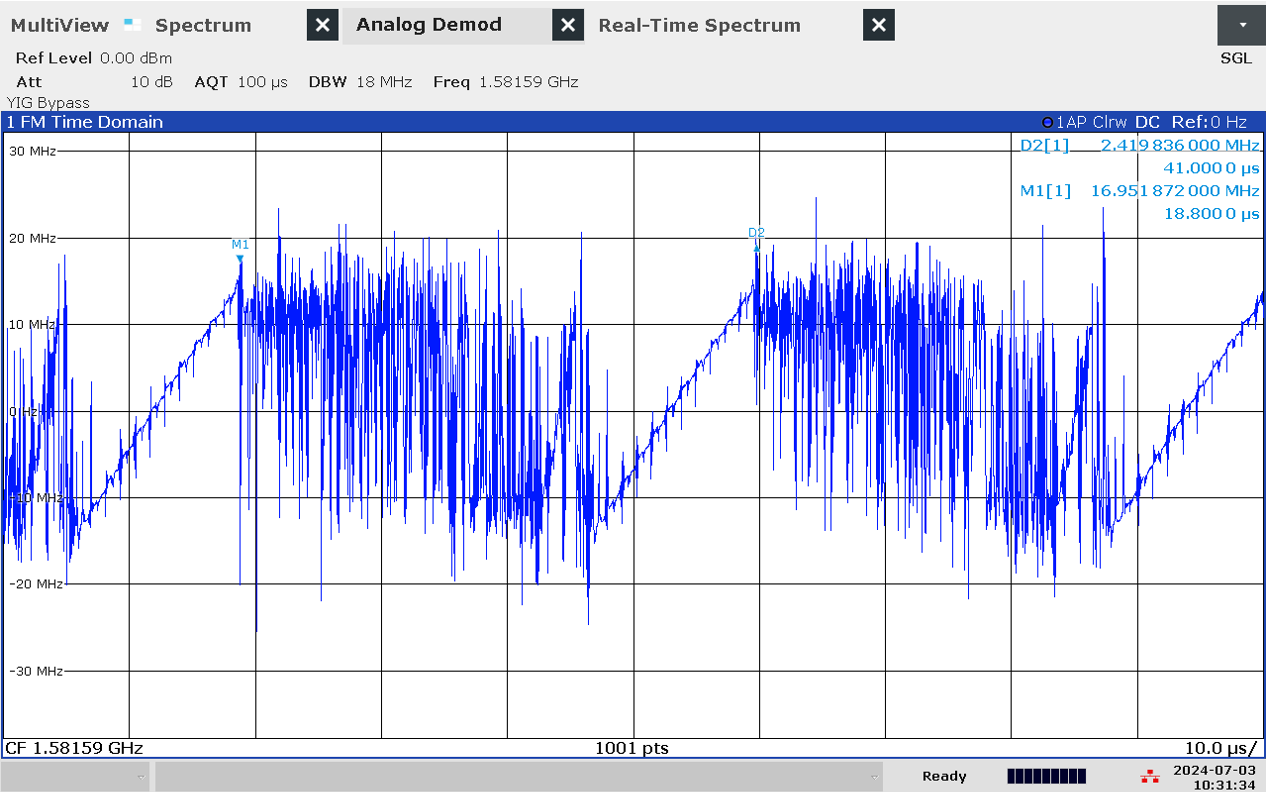
\includegraphics[scale=0.4]{../graphics/appendixG/s2.2-6.png} 
\caption{Time domain (analog demod) measurement of jammer S2.2 on antenna 'L2'}\end{figure}